\chapter[Desenvolvimento da Arquitetura]{Desenvolvimento da Arquitetura}

Este capítulo apresenta o uso de metodologias e conceitos relacionados à Engenharia de Software que aplicados no desenvolvimento descrito no capítulo anterior. Além disto, os testes aplicados e os resultados obtidos são descritos.

A seção 4.1 deste capítulo apresenta uma contextualização da proposta arquitetural implementada. A metodologia de execução, seção 4.2, apresenta aspectos e atividades no processo de desenvolvimento de software adotados para a execução deste projeto de TCC, com detalhes sobre as atividades  e tarefas realizadas. A seção seguinte, Implementação da arquitetura, exibe os detalhes sobre a implementação da arquitetura, incluindo detalhes sobre as atividades desenvolvidas, tais como adaptação de uma aplicação legada, construção de um novo serviço como uma API REST e a integração destes serviços ao ESB e outras aplicações cliente. A última seção, 4.4, apresenta os testes realizados e os resultados coletados.

\section{Introdução}
O projeto de Engenharia de Software desenvolvido como parte do trabalho de conclusão de curso consiste em uma arquitetura para uma plataforma virtual, onde as funcionalidades serão tratadas como serviços no contexto arquitetural. Os serviços ou funcionalidades desta plataforma virtual consistem de aplicações de \textit{software} desenvolvidas no contexto do grupo de orientação e trabalhos desenvolvidos em laboratórios de pesquisa e desenvolvimento de \textit{software} da Universidade de Brasília. A plataforma virtual é um meio de disponibilizar tais trabalhos para uso pela comunidade.

A proposta descrita no capítulo 3 foi desenvolvida utilizando-se de alguns conceitos de metodologia ágil de desenvolvimento e de gerenciamento de projetos de software, adaptadas às necessidades deste projeto.

\section{Metodologia de Execução}
Um projeto de Engenharia de Software deve ser realizado utilizando-se de metodologias, técnicas e ferramentas disponíveis, relacionadas à área de conhecimento, sendo sempre adaptadas de acordo com o projeto a ser desenvolvido visando, assim, o sucesso na conclusão do projeto.

Entre as diversas metodologias de desenvolvimento de software existentes, foi decidido pela adoção de uma metodologia ágil para o desenvolvimento deste projeto. Para a execução, foram praticados conceitos relacionados à metodologia ágil de desenvolvimento, mais especificamente o Scrum. O modelo de desenvolvimento adotado foi iterativo e incremental, tornando a identificação de falhas e correção das mesmas mais eficiente, assim como a identificação de novas necessidades para que a arquitetura e o protocolo de comunicação propostos sejam implementados.

Um dos conceitos ágeis utilizados foi o de histórias de usuário: descrição de funcionalidades que agregam valor ao produto final a ser entregue, escrita de maneira simples e facilmente entendida. As histórias elicitadas consistiram tanto de histórias que descrevem funcionalidades, quando de histórias técnicas, que tratam de adaptação e implantação de tecnologias e outros aspectos relacionados à características técnicas do desenvolvimento de software.

\subsection{Atividades de Execução}
Foram realizadas atividades de adaptação de uma aplicação e a incorporação desta aplicação como um serviço à plataforma virtual foram realizadas de maneira iterativa e incremental. Isto justifica o uso de um método de desenvolvimento de \textit{software} capaz de fornecer suporte para que iterações sejam executadas.

As atividades foram desenvolvidas com base em histórias de usuário e histórias técnicas. Estas histórias foram tratadas como tarefas a serem realizadas para que a atividade pudesse ser completada com êxito. Abaixo estão relacionadas as atividades e as descrições das histórias relacionadas a cada atividade executada.

\begin{itemize}
\item \textbf{Adaptação de uma aplicação já desenvolvida e Testes:} 

\begin{itemize}
\item Eu, como desenvolvedor(a), desejo verificar o escopo e proposta de aplicações já existentes para que eu possa selecionar uma destas transformá-la em um serviço (API REST).
\item Eu, como desenvolvedor(a), desejo analisar o código-fonte disponibilizado da aplicação escolhida para identificar pontos de alteração necessários.
\item Eu, como desenvolvedor(a), desejo construir uma camada REST para disponibilizar o serviço da aplicação escolhida sem  que a sua essência seja modificada.
\end{itemize}

\item \textbf{Análise de ferramentas ESB:} 
\begin{itemize}
\item Eu, como desenvolvedor(a) da arquitetura, desejo testar e analisar as ferramentas ESB levantadas inicialmente para que eu possa selecionar uma delas na implementação da arquitetura.
\end{itemize}

\item \textbf{Implantação da ferramenta escolhida:} 
\begin{itemize}
\item Eu, como desenvolvedor(a) da arquitetura, desejo ter a ferramenta ESB escolhida implantada para que eu possa realizar a integração das aplicações e realizar testes desta integração.
\end{itemize}

\item \textbf{Implementação da plataforma virtual:} 
\begin{itemize}
\item Eu, como usuário do sistema, desejo que o serviço adaptado seja disponibilizado por meio de uma plataforma virtual web para que eu possa utilizá-lo para fins diversos.
\end{itemize}

\item \textbf{Integração de serviços, ESB e plataforma virtual e Testes:} 
\begin{itemize}
\item Eu, como desenvolvedor(a) da arquitetura, desejo realizar a integração a aplicação que foi adaptada e a plataforma virtual através da ferramenta ESB escolhida para que este sirva de modelo para integrações futuras.
\end{itemize}

\item \textbf{Desenvolvimento de API de login e Testes:} 
\begin{itemize}
\item Eu, como desenvolvedor(a) da arquitetura, desejo desenvolver um serviço de login para diversas plataformas e serviços para que usuários de plataformas e serviços da arquitetura sejam gerenciados por este serviço.
\item Eu, como usuário, gostaria de realizar meu cadastro na plataforma virtual para que eu possa usufruir do máximo de serviços da plataforma.
\item Eu, como usuário, gostaria de realizar meu cadastro e login utilizando contas de redes sociais para que eu possa gerenciar mais facilmente minhas contas e usufruir do máximo de serviços da plataforma.
\end{itemize}

\item \textbf{Integração de API de login, ESB e plataforma virtual e Testes:} 
\begin{itemize}
\item Eu, como desenvolvedor(a) da arquitetura, desejo realizar a integração do serviço de login e a plataforma virtual através da ferramenta ESB escolhida para que usuários sejam gerenciados pelo serviço.
\end{itemize}

\end{itemize}

\section{Implementação da Arquitetura}
Foram integradas à arquitetura proposta dois serviços: um de análise de aderência de perfis e outro de gerenciamento de usuários. Os dois serviços foram implementados com o objetivo de demonstrar como adaptar um sistema legado para ser integrado à arquitetura e como desenvolver uma aplicação planejada como um serviço que fornece suas funcionalidades por meio de uma API REST.

Esta seção está subdividida em quatro tópicos principais. O primeiro tópico trata da adaptação de um sistema legado desenvolvido como uma aplicação nativa Java, construindo, a partir do núcleo de funcionalidades da aplicação, uma interface que a transformou em uma API RESTful em Java. O segundo tópico, Construção de um Serviço Gerenciador de Usuários, trata do desenvolvimento da API de gerenciamento de usuários. Detalhes sobre a implementação do ambiente virtual e de como foram realizadas as requisições e tratamento de respostas estão descritos no terceiro tópico. O último, Integração através do ESB, exibe como foi feita a conexão dos serviços ao barramento de serviços utilizado (WSO2 ESB).

\subsection{Adaptação de Aplicação Existente}
Na parte inicial da implementação do protótipo da arquitetura proposta, as atividades realizadas foram a adaptação de uma ferramenta existente para integração de suas funcionalidades como um serviço; a construção de uma plataforma virtual onde os serviços podem ser acessados; e integração da plataforma virtual e do serviço com o auxílio do ESB escolhido. O padrão de comunicação estabelecido faz uso do protocolo REST. O formato de mensagem padrão trocados entre as aplicações através do ESB é o JSON.

A aplicação escolhida para a atividade de adaptação é um algoritmo de análise de aderência de perfis baseado no currículo acadêmico de indivíduos \cite{jesus_algoritmo_2014}. Esta foi a aplicação escolhida devido ao recente desenvolvimento, disponibilidade para contato com o desenvolvedor do algoritmo e disponibilidade do código-fonte da aplicação.

Primeiramente foi realizada a preparação do ambiente para execução da aplicação existente. O ambiente requerido consiste em um ambiente de desenvolvimento Java. As tecnologias utilizadas para a preparação do ambiente de desenvolvimento foram:
\begin{itemize}
\item Java SDK 1.8;
\item Eclipse IDE;
\item Apache Tomcat 7.0;
\item Linux Mint 17.3;
\item framework Jersey 2.24;
\item POSTMAN REST Client.
\end{itemize}

Através de testes dinâmicos (execução da aplicação) e análise estática do código-fonte, foi identificado que esta aplicação utiliza a ontologia gerada por uma ferramenta chamada \textit{scriptLattes}\footnote{Mais sobre \textit{scriptLattes}: http://scriptlattes.sourceforge.net/} . Esta ferramenta realiza o \textit{download} automático do currículo acadêmico disponibilizado em uma plataforma brasileira de pesquisa. Deste currículo, em formato HTML, são extraídas informações sobre produções bibliográficas, técnicas e artísticas, além de orientações, projetos de pesquisa, prêmios, títulos e colaborações \cite{scriptlattes_2009}. Com base nos dados extraídos, o cálculo de aderência de perfis é realizado.

Por ser uma aplicação Java, a proposta para adaptação é a construção de uma API RESTful em Java. Isto ocorreu para que a integridade do o algoritmo inicial fosse mantida. Para a construção da API, foi utilizado o framework Jersey 2.24 \footnote{Sobre o Jersey Framework: https://jersey.java.net/}, que viabiliza o desenvolvimento de \textit{RESTful Web Services} em Java.

Para a disponibilização das funcionalidades da aplicação escolhida por meio de uma API, foram construídas uma operação que acessa o método principal de forma simples e outra operação que permite a comparação de mais de dois currículos. Desta forma, a API disponibiliza o cálculo de aderência de perfis 1:1 e 1:N. Para a realização do cálculo de aderência de perfis, as informações e os formatos de mensagem a ser enviado são demonstrados pelos Códigos \ref{lst:msgrecebida11} e \ref{lst:msgrecebida1N}.


\definecolor{verde}{rgb}{0.25,0.5,0.35}
\definecolor{jpurple}{rgb}{0.5,0,0.35}

\lstset{
  language=Java,
  basicstyle=\ttfamily\small, 
  keywordstyle=\color{jpurple}\bfseries,
  stringstyle=\color{blue},
  commentstyle=\color{verde},
  extendedchars=true, 
  showspaces=false, 
  showstringspaces=false, 
  numbers=left,
  numberstyle=\tiny,
  breaklines=true, 
  backgroundcolor=\color{cyan!10}, 
  breakautoindent=true, 
  captionpos=b,
  xleftmargin=0pt,
  tabsize=4,
  texcl=true
}
\begin{lstlisting}[caption={Formato de mensagem recebido pela API (1:1).},label={lst:msgrecebida11}]
{
"individuo_base":{
         "nome_base":"<nome_base_como_no_curriculo_lattes>",
         "id_base":"<id_como_no_curriculo_lattes>"
            },
"individuo_destino":{
     "nome_destino":"<nome_como_no_curriculo_lattes>",
     "id_destino":"<id_como_no_curriculo_lattes>"
            },
"cv_base":"<arquivo_como_grande_string>",
"cv_destino":"<arquivo_como_grande_string>"
}
\end{lstlisting}


\definecolor{verde}{rgb}{0.25,0.5,0.35}
\definecolor{jpurple}{rgb}{0.5,0,0.35}

\lstset{
  language=Java,
  basicstyle=\ttfamily\small, 
  keywordstyle=\color{jpurple}\bfseries,
  stringstyle=\color{blue},
  commentstyle=\color{verde},
  extendedchars=true, 
  showspaces=false, 
  showstringspaces=false, 
  numbers=left,
  numberstyle=\tiny,
  breaklines=true, 
  backgroundcolor=\color{cyan!10}, 
  breakautoindent=true, 
  captionpos=b,
  xleftmargin=0pt,
  tabsize=4,
  texcl=true
}
\begin{lstlisting}[caption={Formato de mensagem recebido pela API (1:N).},label={lst:msgrecebida1N}]
{
"individuo_base":{
	        	 "nome_base":"<nome_base_como_no_curriculo_lattes>",
    		     "id_base":"<id_como_no_curriculo_lattes>"
	            },
"individuos_destino":{
				"<nome1>":"<id_curriculo_lattes_01>",
				"<nomeX>":"<id_curriculo_lattes_0X>"
				},
"cv_base":"<arquivo_como_grande_string>",
"cvs_destino":{
				"<nome1>":"<arquivo_como_grande_string>",
				"<nomeX>":"<arquivo_como_grande_string>"
				}
}
\end{lstlisting}

O nome completo, código identificador do currículo e arquivo do currículo devem ser enviados na mensagem escrita no formato JSON. Devido ao impedimento de download automático do currículo acadêmico causado pelo uso de \textit{captchas}, a ferramenta \textit{scriptLattes} foi adaptada para execução local. Para tanto, se faz necessário o recebimento do currículo acadêmico em formato HTML, nome conforme informado no currículo e o código identificar correspondente.

A partir de tais informações, os nomes dos indivíduos são fornecidos ao código de aderência de perfis. Os resultados finais são enviados como resposta e contém os nomes dos indivíduos e o percentual de aderência. A mensagem de resposta também é no formato JSON. Assim, os formatos de mensagens de resposta para os cálculos de aderência 1:1 e 1:N são exibidos nos Códigos \ref{lst:msgresposta11} e \ref{lst:msgresposta1N}.


\definecolor{verde}{rgb}{0.25,0.5,0.35}
\definecolor{jpurple}{rgb}{0.5,0,0.35}

\lstset{
  language=Java,
  basicstyle=\ttfamily\small, 
  keywordstyle=\color{jpurple}\bfseries,
  stringstyle=\color{blue},
  commentstyle=\color{verde},
  extendedchars=true, 
  showspaces=false, 
  showstringspaces=false, 
  numbers=left,
  numberstyle=\tiny,
  breaklines=true, 
  backgroundcolor=\color{cyan!10}, 
  breakautoindent=true, 
  captionpos=b,
  xleftmargin=0pt,
  tabsize=4,
  texcl=true
}
\begin{lstlisting}[caption={Formato de mensagem de resposta(1:1).},label={lst:msgresposta11}]
{
"individuo_base":{
         "nome_base":"<nome_base_como_no_curriculo_lattes>",
         "id_base":"<id_como_no_curriculo_lattes>"
            },
"individuo_destino":{
     "nome_destino":"<nome_como_no_curriculo_lattes>",
     "id_destino":"<id_como_no_curriculo_lattes>"
            },
"percentual_aderencia":"<valor_calculado_em_porcentagem>",
"equivalencias":{
				"<titulo1>":[<titulo_destino_equivalente1>,...,<titulo_destino_equivalenteN>],
				"<tituloN>":[<titulo_destino_equivalente1>,...,<titulo_destino_equivalenteN>],
				}
}


\end{lstlisting}


\definecolor{verde}{rgb}{0.25,0.5,0.35}
\definecolor{jpurple}{rgb}{0.5,0,0.35}

\lstset{
  language=Java,
  basicstyle=\ttfamily\small, 
  keywordstyle=\color{jpurple}\bfseries,
  stringstyle=\color{blue},
  commentstyle=\color{verde},
  extendedchars=true, 
  showspaces=false, 
  showstringspaces=false, 
  numbers=left,
  numberstyle=\tiny,
  breaklines=true, 
  backgroundcolor=\color{cyan!10}, 
  breakautoindent=true, 
  captionpos=b,
  xleftmargin=0pt,
  tabsize=4,
  texcl=true
}
\begin{lstlisting}[caption={Formato de mensagem de resposta (1:N).},label={lst:msgresposta1N}]
{
"individuo_base":{
         "nome_base":"<nome_base_como_no_curriculo_lattes>",
         "id_base":"<id_como_no_curriculo_lattes>"
         },
"<idbase_iddestino1>":{
		"percentual_aderencia":"<valor_calculado_em_porcentagem>",
		"individuo_destino1":{
						     "nome_destino":"<nome_como_no_curriculo_lattes>",
						     "id_destino":"<id_como_no_curriculo_lattes>"
				            },
		"equivalencias":{
				"<titulo1>":[<titulo_destino_equivalente1>,...,<titulo_destino_equivalenteN>],
				"<tituloN>":[<titulo_destino_equivalente1>,...,<titulo_destino_equivalenteN>],
				}
	},
"<idbase_iddestinoN>":{
		"percentual_aderencia":"<valor_calculado_em_porcentagem>",
		"individuo_destinoN":{
						     "nome_destino":"<nome_como_no_curriculo_lattes>",
						     "id_destino":"<id_como_no_curriculo_lattes>"
				            },
		"equivalencias":{
				"<titulo1>":[<titulo_destino_equivalente1>,...,<titulo_destino_equivalenteN>],
				"<tituloN>":[<titulo_destino_equivalente1>,...,<titulo_destino_equivalenteN>],
				}
	}
}
\end{lstlisting}

As mensagens de resposta contém o nome e o código identificador do currículo dos indivíduos, o valor do percentual de aderência obtido e uma lista de equivalências de publicações. Como as análises são realizadas com base nas produções bibliográficas, técnicas e artísticas, orientações, projetos de pesquisa, prêmios, títulos e colaborações é possível parear as equivalências destes artefatos entre os indivíduos. Esta também foi uma modificação realizada, cujo objetivo é fornecer ao usuário não somente um percentual, mas identificar produções em temas de interesse mútuo. Estas informações também estão inclusas na mensagem de resposta a ser enviada.

Os testes de envio de requisição e verificação de respostas obtidas foram realizados com o uso do aplicativo Postman REST Client\footnote{Mais sobre Postman: https://www.getpostman.com/}. Esta ferramenta é utilizada como um aplicativo no Google Chrome e colabora na realização de testes de APIs RESTful. O app Postman permite que requisições sejam facilmente construídas, permitindo assim que APIs RESTful sejam testadas sem a necessidade de construir uma aplicação cliente apenas para a execução de testes da API desenvolvida.

A API RESTful construída a partir da aplicação já existente foi implantada em um servidor de aplicações (Apache Tomcat 7.0). Desta forma, foi disponibilizada e pôde ser testada e, posteriormente, conectada ao barramento de serviços escolhido (WSO2 ESB).

\subsection{Construção do Serviço Gerenciador de Usuários}
Um serviço para gerenciamento de usuários foi construído com o intuito de controlar o acesso de usuários às aplicações cliente e serviços conectados ao barramento de serviços e demonstrar a integração de uma aplicação nova, planejada para fornecer suas funcionalidades como serviço. Este serviço armazena informações de usuários e quais as aplicações que o usuário possui permissão de acesso. Desta forma, o acesso a serviços contidos em uma mesma aplicação cliente pode ser gerenciado por meio deste terceiro serviço.

As tecnologias utilizadas para o desenvolvimento da API de gerenciamento de usuários foram:
\begin{itemize}
\item Python 3.4;
\item Django 1.9;
\item Django REST framework (versão 3);
\item PyCharm IDE;
\item Linux Mint 17.3.
\end{itemize}

A API de gerenciamento de usuários desenvolvida possui três das operações básicas do protocolo HTTP: GET, POST e PUT. Para cada uma destas operações dispõe de um método correspondente. O método GET não recebe parâmetros no corpo da mensagem: os parâmetros são parte da URL e, a partir do nome de usuário e do nome identificador de uma aplicação ou serviço, retorna se o usuário possui autorização de acesso à aplicação ou serviço. O registro de usuários e a associação ao serviço ou aplicação é feito por meio do método POST: o corpo da mensagem JSON contém os dados do usuário e o nome que identifica a aplicação ou serviço. O método PUT foi desenvolvido para que os dados do usuário possam ser atualizados.

\definecolor{verde}{rgb}{0.25,0.5,0.35}
\definecolor{jpurple}{rgb}{0.5,0,0.35}

\lstset{
  language=Java,
  basicstyle=\ttfamily\small, 
  keywordstyle=\color{jpurple}\bfseries,
  stringstyle=\color{blue},
  commentstyle=\color{verde},
  extendedchars=true, 
  showspaces=false, 
  showstringspaces=false, 
  numbers=left,
  numberstyle=\tiny,
  breaklines=true, 
  backgroundcolor=\color{cyan!10}, 
  breakautoindent=true, 
  captionpos=b,
  xleftmargin=0pt,
  tabsize=4,
  texcl=true
}
\begin{lstlisting}[caption={Formato de mensagem recebido pelo serviço de gerenciamento de usuários (método POST).},label={lst:msgloginpost}]
{
"usuario":{
	"first_name":"<primeiro_nome>",
	"last_name":"<sobrenome>",
	"username":"<nome_de_usuario>",
	"password":"<senha>",
	"email":"<email>"
	},
"aplicacao":"<nome_aplicacao>"
}
\end{lstlisting}

\definecolor{verde}{rgb}{0.25,0.5,0.35}
\definecolor{jpurple}{rgb}{0.5,0,0.35}

\lstset{
  language=Java,
  basicstyle=\ttfamily\small, 
  keywordstyle=\color{jpurple}\bfseries,
  stringstyle=\color{blue},
  commentstyle=\color{verde},
  extendedchars=true, 
  showspaces=false, 
  showstringspaces=false, 
  numbers=left,
  numberstyle=\tiny,
  breaklines=true, 
  backgroundcolor=\color{cyan!10}, 
  breakautoindent=true, 
  captionpos=b,
  xleftmargin=0pt,
  tabsize=4,
  texcl=true
}
\begin{lstlisting}[caption={Formato de mensagem recebido pelo serviço de gerenciamento de usuários (método PUT).},label={lst:msgloginput}]
{
"first_name":"<primeiro_nome>",
"last_name":"<sobrenome>",
"username":"<nome_de_usuario>",
"password":"<senha>",
"email":"<email>"
}
\end{lstlisting}

Os Códigos \ref{lst:msgloginpost} e \ref{lst:msgloginput} exibem os formatos de mensagem aceitos pelos métodos POST e PUT da API construída. Conforme exposto, o método PUT, no estado atual da API, recebe apenas dados para atualização do registro do usuário. O método POST, recebe dados para registro do usuário, bem como o nome identificador do serviço ou aplicação.

\subsection{Construção do Ambiente Virtual}
O ambiente virtual foi construído com o propósito de implementar uma aplicação \textit{front-end} para usufruto de serviços disponibilizados e conectados ao barramento de serviços. O ambiente virtual é o elemento responsável pela coleta de dados necessários para a execução de um serviço. O envio destes dados é por meio de uma requisição ao ESB. Este componente arquitetural é também responsável por exibir resultados obtidos nas respostas recebidas dos serviços. Para o usuário, o uso de serviços externos ao ambiente virtual é transparente. Isto significa que o usuário final não distingue se a operação é realizada pelo ambiente virtual ou por um serviço externo à esta plataforma.

Para o desenvolvimento, optou-se pelo uso da linguagem de programação Python (3.4). Esta linguagem de programação possui frameworks que permitem a construção de plataformas para web. O framework escolhido é conhecido como Django (versão 1.9). O ambiente de desenvolvimento foi estabelecido com o sistema operacional Linux Mint (17.3). A construção do código-fonte foi realizado com o auxílio da IDE para Python chamada PyCharm IDE.

Uma das estruturas de dados suportadas pela linguagem de programação Python é o dicionário. Esta estrutura define pares chave-valor e pode ser facilmente manipulada. Como a estrutura JSON também consiste de pares chave-valor, os dados das requisições são construídos no formato de um dicionário e convertido para JSON.

Existe uma variedade de bibliotecas disponíveis para uso no desenvolvimento de sistemas de software em Django. Como o desenvolvimento desta plataforma será contínua assim como a produção de software no contexto definido, a existência de diversas bibliotecas colabora e estimula a evolução da mesma. Python dispõe da biblioteca Request (http://docs.python-requests.org/en/master/). Esta biblioteca facilita a implementação de requisições HTTP de todos os tipos (GET, POST, PUT, DELETE, OPTIONS) realizadas em aplicações Python. Para realizar uma requisição simples é necessário definir a URL, dados de cabeçalho e valores do corpo da mensagem (\textit{payload}) (Código \ref{lst:requisicaopython}).

\definecolor{verde}{rgb}{0.25,0.5,0.35}
\definecolor{jpurple}{rgb}{0.5,0,0.35}

\lstset{
  language=Python,
  basicstyle=\ttfamily\small, 
  keywordstyle=\color{jpurple}\bfseries,
  stringstyle=\color{blue},
  commentstyle=\color{verde},
  extendedchars=true, 
  showspaces=false, 
  showstringspaces=false, 
  numbers=left,
  numberstyle=\tiny,
  breaklines=true, 
  backgroundcolor=\color{cyan!10}, 
  breakautoindent=true, 
  captionpos=b,
  xleftmargin=0pt,
  tabsize=4,
  texcl=true
}
\begin{lstlisting}[caption={Requisição HTTP em Python utilizando a biblioteca Request.},label={lst:requisicaopython}]
def calcula_aderencia_simples():
    url = "http://localhost:8280/aderencia/simples"
    cabecalho = {'Content-type': 'application/json'}
    ...
    requests.post(url, data=json.dumps(conteudo), headers=cabecalho, timeout=6000)
\end{lstlisting}

O Código \ref{lst:requisicaopython} representa o código-fonte do \textit{backend} de uma requisição realizada no ambiente virtual para uso do serviço disponibilizado no barramento de serviços do ESB. A url representa o endereço de acesso ao serviço. O cabeçalho deve conter a operação requisitada ao serviço. Os valores do corpo da mensagem contém os parâmetros requisitados pelo serviço para que este possa executar a operação desejada.

A requisição realizada retorna uma resposta. As principais informações contidas na mensagem de resposta são o conteúdo e o código de status da mensagem. O conteúdo pode ser um texto ou um JSON com dados de resposta enviados pelo serviço. O status da mensagem informa se a requisição foi aceita com sucesso ou contém erros, além de indicar a inexistência da operação ou serviço ou a não autorização para acesso.

Uma vez realizada a requisição, o ambiente virtual é o componente arquitetural responsável por exibir o conteúdo da mensagem de resposta do serviço ao usuário. Os valores contidos na mensagem de resposta é especificado no contrato de serviços da aplicação. No caso implementado, a resposta obtida está no formato JSON e os identificadores (chaves) de cada valor são conhecidos. Desta forma, o ambiente virtual trata o payload de resposta como um dicionário e os valores obtidos são exibidos ao usuário final da plataforma \textit{web} (ver Figura \ref{print_ambiente_virtual}).

\begin{figure}[!hbt]
\centering
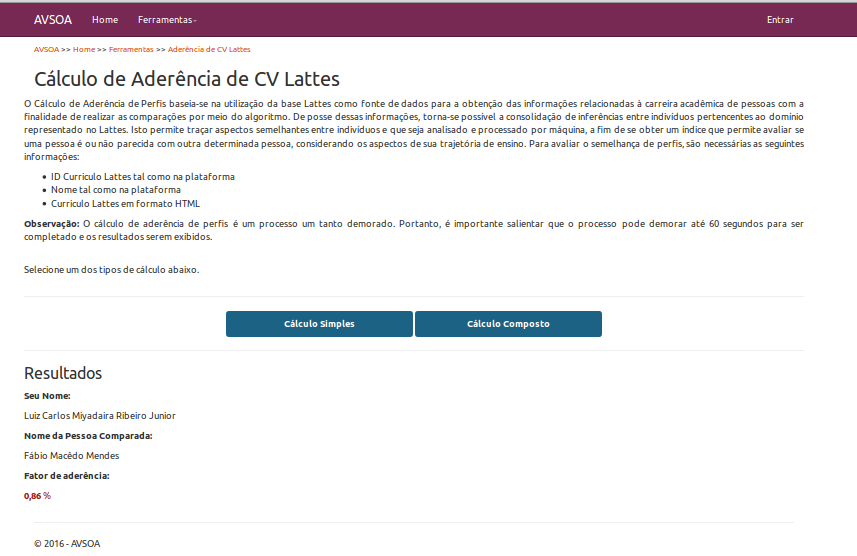
\includegraphics[scale=0.7]{figuras/print_avsoa.png}
\caption{Dados exibidos no Ambiente Virtual.}
\label{print_ambiente_virtual}
\end{figure}

A Figura \ref{print_ambiente_virtual} exibe um exemplo de uma aplicação \textit{front-end} renderizando e exibindo os dados obtidos através de uma requisição realizada. Os dados da requisição realizada para o serviço de cálculo de aderência de perfis são dispostos como exibido na Figura \ref{print_ambiente_virtual}. Contudo, tais dados poderiam ser exibidos de uma maneira diferente, inclusive mostrando os resultados de equivalências entre produções bibliográficas, técnicas e artísticas, orientações, projetos de pesquisa, prêmios, títulos e colaborações dos indivíduos em questão.

\subsection{Integração através do ESB}
A arquitetura SOA implementada utilizou a abordagem de integração Hub-and-Spoke. Para a implementação desta abordagem é necessário o uso de um barramento de serviços. O barramento escolhido neste estudo de caso foi o WSO2 ESB, devido ao fato de este atender aos critérios de seleção estabelecidos. 

Este barramento de serviços oferece as opções de adicionar o serviço como um serviço de \textit{proxy} \footnote{Serviços \textit{Proxy} no WSO2 ESB: https://docs.wso2.com/display/ESB480/Working+with+Proxy+Services} e também como uma API. O serviço de \textit{proxy} é um recurso fornecido pelo WSO2 ESB que recebe mensagens de requisição de serviços e pode processar a mensagem antes de redirecionar ao serviço. Os fluxos de mensagens de requisição e de resposta são tratados pelo serviço de \textit{proxy}. Este recurso permite a introdução de novas funcionalidades ao serviço sem alterá-lo. O tratamento de requisições pode definir respostas sem mesmo entregar as requisições aos serviços. O WSO2 ESB também permite a exposição de APIs RESTful e a mediação de requisições realizadas no ESB. O uso de WSO2 ESB REST API permite a configuração direta de \textit{end-points} com a especificação de uma operação HTTP, URI \textit{template} e URI \textit{mappings}. Estes componentes de URI definem a URL de acesso à operação/serviço.

O serviço adicionado ao barramento consiste de uma aplicação que realiza o cálculo da aderência de perfis de usuários. Este serviço fornece suas operações por meio de uma API RESTful e está implantado em um servidor de aplicações externo (Tomcat 7.0). As operações deste serviço podem ser adicionadas tanto como um serviço de \textit{proxy}, quanto como uma API ao barramento. Em ambos os casos será gerado uma URL de acesso ao serviço e suas operações. Por se caracterizar em um API, o serviço foi adicionado ao barramento como tal. Ao adicionar uma API ao barramento, o endereço de acesso aos recursos definidos pela API REST pode ser modificado. Esta modificação tem como finalidade simplificar grandes URLs de acesso ou até mesmo eliminar a necessidade de dados padrões que são definidos na própria URL.

Para a adição do serviço como API ao WSO2 ESB, cada operação da API é definida como um recurso ou operação. O serviço de cálculo de aderência de currículo adicionado possui duas operações. As operações seguem o mesmo padrão de execução quando as requisições são realizadas. A diferença é o modo como o conteúdo das mensagens estão organizadas. Abaixo está o modelo de código XML gerado ao adicionar a API como um serviço no ESB.

\definecolor{verde}{rgb}{0.25,0.5,0.35}
\definecolor{jpurple}{rgb}{0.5,0,0.35}

\lstset{
  language=XML,
  basicstyle=\ttfamily\small, 
  keywordstyle=\color{jpurple}\bfseries,
  stringstyle=\color{blue},
  commentstyle=\color{verde},
  extendedchars=true, 
  showspaces=false, 
  showstringspaces=false, 
  numbers=left,
  numberstyle=\tiny,
  breaklines=true, 
  backgroundcolor=\color{cyan!10}, 
  breakautoindent=true, 
  captionpos=b,
  xleftmargin=0pt,
  tabsize=4,
  texcl=true
}
\begin{lstlisting}[caption={Código XML gerado pelo WSO2ESB durante o \textit{deploy} da API REST.} ,label={lst:xmldeployapi}]
<api xmlns="http://ws.apache.org/ns/synapse" name="AderenciaPerfilLattes" context="/aderencia">
   <resource methods="POST" url-mapping="/simples">
      <inSequence>
         <property name="content-type" value="application/json" scope="default"/>
         <send>
            <endpoint>
               <http method="POST" uri-template="<URL_da_operacao_do_servico>"/>
            </endpoint>
         </send>
      </inSequence>
      <outSequence>
         <send/>
      </outSequence>
   </resource>
   <resource methods="POST" url-mapping="/composta">
      <inSequence>
         <property name="content-type" value="application/json" scope="default"/>
         <send>
            <endpoint>
               <http method="POST" uri-template="<URL_da_operacao_do_servico>"/>
            </endpoint>
         </send>
      </inSequence>
      <outSequence>
         <send/>
      </outSequence>
   </resource>
</api>
\end{lstlisting}

Este modelo apresenta os passos a serem seguidos pela ferramenta quando uma requisição é feita para a API que realiza o cálculo de aderência de perfis. As requisições feitas para ambas operações fornecidas pelo serviço são identificadas como um recurso. As requisições realizadas são do tipo POST porque o recebimento de dados no conteúdo da mensagem só é permitido quando é realizada esta operação. Esta é uma restrição do framework Jersey utilizado para a construção da API RESTfull do serviço de cálculo de aderência de perfis de usuários. O valor “\textit{url-mapping}” define o nome reconhecido pelo ESB da operação do serviço requisitada.

A sequência de entrada (\textit{inSequence}) estabelece os passos serem seguidos quando uma requisição é recebida pelo ESB. Aqui conversões de formatos de mensagens e adaptações entre protocolos podem ser realizados. Neste caso, o ESB deve redirecionar o \textit{payload} da mensagem diretamente à URL indicada na \textit{tag} <http>. A sequência de saída (\textit{outSequence}) define o que deve ser feito quando a resposta correspondente à requisição é recebida pelo ESB. Novamente, as mensagens podem ser tratadas, convertidas, salvas, clonadas e redirecionadas também para outros serviços ou aplicações cliente. A sequência de saída definida ao adicionar o serviço de cálculo de aderência de currículo apenas redireciona a resposta recebida ao ambiente virtual. Sequências para casos de falhas (\textit{faultSequence}) também podem ser definidas.

O serviço não é capaz de distinguir quando uma requisição é realizada por uma conexão ponto a ponto entre aplicações ou quando é realizada por um software intermediário como o ESB. Enquanto isto, o usuário desconhece o mecanismo de execução de tal serviço.

O ambiente virtual desenvolvido implementa o \textit{front-end} do serviço: os dados são capturados nesta plataforma \textit{web} e em seguida a requisição ao serviço do ESB é enviada. A Figura  \ref{integracao_esb_front_rest_api_tcc} ilustra a integração de serviços e componentes de \textit{software}.

\begin{figure}[!hbt]
\centering
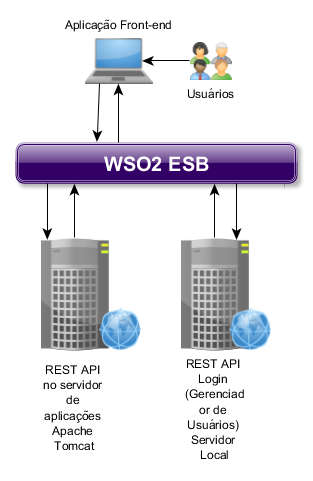
\includegraphics[scale=0.7]{figuras/integracao_esb_front_rest_api_tcc.png}
\caption{Ilustração da integração final obtida.}
\label{integracao_esb_front_rest_api_tcc}
\end{figure}

A Figura \ref{integracao_esb_front_rest_api_tcc} apresenta os componentes e o fluxo de mensagens de requisições e resposta. A comunicação é iniciada quando o usuário fornece os dados necessários e solicita o serviço informado. O ambiente virtual trata estas informações, as organiza e identifica conforme o solicitado no contrato de serviços e realiza a requisição. O ESB redireciona esta requisição ao serviço correspondente, indicado pela URL. A resposta obtida pelo ESB é redirecionada ao ambiente virtual.

\subsubsection{Construção de conector}
Um conector facilita a interação entre aplicações cliente e operações fornecidas por serviços, permitindo que estes clientes interajam com APIs de serviços como Google+, Facebook e GitHub \cite{wso2}. Para a conexão com a API de gerenciamento de usuários e aplicações, foi criado um conector que trata a mensagem recebida, ajusta os dados da mensagem para o formato correto e envia a requisição para a API. O conector foi construído com base na documentação da ferramentas WSO2 ESB\footnote{Instruções em: https://docs.wso2.com/display/ESBCONNECTORS/Writing+a+Connector}. O código do conector está disponível no Apêndice A deste documento.

As operações do serviço oferecido pela API de gerenciamento de usuários foram adicionadas ao ESB por meio da adição de um serviço de proxy, recebendo as mensagens, identificando a operação e conectando ao serviço utilizando o conector produzido. 

O serviço de \textit{proxy} é um recurso fornecido pelo WSO2 ESB que recebe mensagens de requisição de serviços e pode processar a mensagem antes de redirecionar ao serviço. Os fluxos de mensagens de requisição e de resposta são tratados pelo serviço de \textit{proxy}. Este recurso permite a introdução de novas funcionalidades ao serviço sem alterá-lo. O tratamento de requisições pode definir respostas sem mesmo entregar as requisições aos serviços. Segue a definição do serviço de proxy criado.


\definecolor{verde}{rgb}{0.25,0.5,0.35}
\definecolor{jpurple}{rgb}{0.5,0,0.35}

\lstset{
  language=XML,
  basicstyle=\ttfamily\small, 
  keywordstyle=\color{jpurple}\bfseries,
  stringstyle=\color{blue},
  commentstyle=\color{verde},
  extendedchars=true, 
  showspaces=false, 
  showstringspaces=false, 
  numbers=left,
  numberstyle=\tiny,
  breaklines=true, 
  backgroundcolor=\color{cyan!10}, 
  breakautoindent=true, 
  captionpos=b,
  xleftmargin=0pt,
  tabsize=4,
  texcl=true
}
\begin{lstlisting}[caption={Código XML de definição de serviço proxy de gerenciamento de usuários.} ,label={lst:xmlproxylogin}]
<?xml version="1.0" encoding="UTF-8"?>
<proxy xmlns="http://ws.apache.org/ns/synapse"
       name="loginConnector"
       startOnLoad="true"
       statistics="enable"
       trace="enable"
       transports="http,https">
   <target>
      <inSequence>
         <log level="full"/>
         <property expression="json-eval($.username)" name="username"/>
         <property expression="json-eval($.client_name)" name="client_name"/>
         <property expression="json-eval($.aplicacao)" name="aplicacao"/>
         <property expression="json-eval($.password)" name="password"/>
         <property expression="json-eval($.first_name)" name="first_name"/>
         <property expression="json-eval($.last_name)" name="last_name"/>
         <property expression="json-eval($.email)" name="email"/>
         <switch source="get-property('transport', 'Action')">
            <case regex="getAuth">
               <login.getAuth>
                  <username>{$ctx:username}</username>
                  <client_name>{$ctx:client_name}</client_name>
               </login.getAuth>
            </case>
            <case regex="saveUser">
               <login.saveUser>
                  <username>{$ctx:username}</username>
                  <password>{$ctx:password}</password>
                  <first_name>{$ctx:first_name}</first_name>
                  <last_name>{$ctx:last_name}</last_name>
                  <email>{$ctx:email}</email>
                  <aplicacao>{$ctx:aplicacao}</aplicacao>
               </login.saveUser>
            </case>
            <case regex="updateUser">
               <login.updateUser>
                  <username>{$ctx:username}</username>
                  <password>{$ctx:password}</password>
                  <first_name>{$ctx:first_name}</first_name>
                  <last_name>{$ctx:last_name}</last_name>
                  <email>{$ctx:email}</email>
               </login.updateUser>
            </case>
         </switch>
         <respond/>
      </inSequence>
      <outSequence>
         <property name="DISABLE_CHUNKING" scope="axis2" value="true"/>
         <log/>
         <send/>
      </outSequence>
   </target>
   <description>Este servico e um gerenciador de autorizacoes de acesso a aplicacoes.
   Action (getAuth): verifica se o usuario esta autorizado a acessar a aplicacao. Parametros: username e client_name.
   Action (saveUser): salva usuario e o associa a aplicacao. Parametros: username, password, email, first_name, last_name, aplicacao.
   Action (updateUser): atualiza dados do usuario (se existir). Parametros: username, password, email, first_name, last_name.
   </description>
</proxy>
\end{lstlisting}

O Código \ref{lst:xmlproxylogin} exibe a definição do serviço de \textit{proxy} de gerenciamento de usuários em XML. O código é gerado pela ferramenta WSO2 ESB ao definir as ações do serviço. O código pode ser alterado pelo desenvolvedor/manutenedor da arquitetura definida.

A definição do serviço de \textit{proxy} estabelece que o serviço permite conexão via protocolos HTTP e HTTPS, além de definir parâmetros necessários, as operações (\textit{Action}) permitidas e o que deve ser feito quando cada operação é acionada. O serviço de \textit{proxy} define também a sequência de saída da mensagem retornada pelo serviço (API REST).

Integrado à plataforma virtual, o serviço de gerenciamento de usuários permite controlar o acesso de usuários aos serviços conectados e disponibilizados através da plataforma. Desta maneira, ao registrar um usuário na plataforma virtual, os dados do usuário são salvos e este é associado à plataforma por meio do seu identificador (método POST da API). Ao tentar realizar o login do usuário na plataforma virtual, é realizada uma requisição afim de verificar se o usuário possui permissão de acesso a plataforma (método GET da API).

\section{Testes e Resultados}
Foram realizadas medições de complexidade, desempenho e esforço empreendido no que diz respeito ao serviço de cálculo de aderência de perfis. Com o auxílio da ferramenta CkeckStyle (http://checkstyle.sourceforge.net/), a complexidade ciclomática do projeto de algoritmo de inferência foi coletada e analisada. A coleta foi realizada antes e depois da adaptação. Como resultado, apenas dois métodos apresentaram complexidade ciclomática alta (acima de 10). Como houve alteração para que a comparação de perfis pudesse ser realizadas no modo 1:N, a complexidade ciclomática do método principal do cálculo de aderência aumentou em uma unidade. Não houve alteração no valor da complexidade ciclomática de outros métodos e classes, uma vez que não foram alteradas ou as alterações não influenciaram nesta medição.

Os testes de desempenho executados compararam esta medida quando o serviço e a aplicação cliente são conectadas ponto a ponto, e quando são conectadas com o uso do WSO2 ESB. Estes testes foram realizados de duas maneiras: na primeira, os testes foram iniciados e as requisições foram enviadas em sequência, sem que nenhum dos componentes (API, ESB ou ambiente virtual) fossem reinicializados (Cenário 1); na segunda, os componentes eram reinicializados antes do envio de uma requisição (Cenário 2). Foi adotado esse método de comparação afim de verificar alterações quando um componente já teve uma operação executada ou dados da execução anterior armazenados em cache. A Tabela \ref{resultado_desempenho} exibe os resultados obtidos.

\begin{table}[!htbp]
\centering
\caption{Resultados de Teste de Desempenho - Cálculo de Aderência de Perfis}
\label{resultado_desempenho}
\begin{tabular}{*5c}
\toprule
  & \multicolumn{2}{c}{Cenário 1} & \multicolumn{2}{c}{Cenário 2} \\ 
\midrule
Número do Teste               & ESB   & Ponto-a-Ponto & ESB    & Ponto-a-Ponto \\
1                            & 97.8  &    103.2      & 107.4  &  123.9   \\
2                            & 100.6 &     97.6      & 103.6  &  101.7   \\
3                            & 96.1  &    104.2      & 107.9  &  105.5   \\ 
4                            & 95.0  &    102.9      &  94.6  &  101.0   \\ 
5                            & 105.6 &     98.7      &  95.2  &   94.8   \\ 
\midrule
\textbf{Média}               & 98.17 &    101.6      & 102.07 &  102.73   \\ 
\bottomrule
\end{tabular}
\end{table}

Os testes de desempenho executados demonstraram que a média de tempo para obtenção de resposta ao requisitar o cálculo do fator de aderência foi maior quando a conexão foi realizada ponto a ponto. Os maiores e menos valores de cada coluna foram excluídos para o cálculo do valor médio final. O resultado dos testes de desempenho executados indica que a proposta arquitetural, como o uso do ESB, não degrada o desempenho geral da solução.

A coleta de esforço empreendido para adaptar a aplicação existente e fornecer suas funcionalidades como serviço através de uma API REST foi realizada com base em \textit{commits} da ferramentas de controle utilizada (Git). Uma vez que os \textit{commits} permitem o registro de modificações e data correspondentes. Esta funcionalidade da ferramenta de controle utilizada foi útil para realizar as medidas de esforço empreendido para implementar a adaptação necessária no código-fonte da aplicação.

O esforço foi medido em tempo e categorizado por dois aspectos: esforço/tempo necessário para adaptação e esforço/tempo empreendido para integração ao barramento de serviços (WSO2 ESB). A medida de esforço para adaptação expressa o tempo utilizado para realizar modificações necessárias no código-fonte e fornecer suas funcionalidades como operações de um serviço em uma API REST. O esforço empreendido para integração ao barramento de serviços mede o tempo (em horas) necessário para a configuração de uma nova aplicação ao incorporá-la como uma API REST ao ESB e implementação do \textit{backend} de uma aplicação cliente (neste caso, o ambiente virtual).

O tempo total de esforço para a adaptação da aplicação foi de 41 horas onde:
\begin{itemize}
\item 5 horas - reconhecimento do código;
\item 6 horas - planejamento de atividades e refatoração inicial;
\item 30 horas - criação da camada de conexão e tratamento de dados da API REST.
\end{itemize}

A construção da plataforma virtual e conexão com o serviço através do ESB consumiu 15 horas de esforço. Desta forma, o esforço total necessário para a adaptação de uma aplicação existente, implementando uma API REST, configuração da API implementada e conexão com uma aplicação cliente foi de 56 horas.
